\section{Dataset of Plastic Soup images}
\label{sec:Data}
Because for this project no dataset was available that consists of labelled images of floating plastic, one was constructed by hand.

The dataset used in this project was created from short films by Bill MacDonnald\footnote{The videos are online on youtube: \url{www.youtube.com/007bmac}. Thank you Bill for letting me use your films in this research}.
Several of these clips consist of floating plastic from a viewpoint both above and below water.
There were also clips that showed the presence of animals.
These clips were segmented in single frames and selected for use in this project; images that did not fall in one of the four classes (plastic, animals, both or none) were excluded.
A total of 37.165 images were left to annotate.
The annotation was done by my hand, classifying each image on viewpoint and if plastic or animals were visible.
To facilitate the annotation, a small Java-application was made.
With the use of several key-strokes, large amounts of image-data could be annotated with relative ease.
Even so, the annotation of the data took a considerable amount of time.

In total 20.635 images showed plastic only, 6.972 images showed animals only and 8.502 images show both.
The above (16.553) and below (20.612) viewpoints were separated into two datasets, to both train and test separately. 
In the above-set, a total of 14.588 images showed plastic, 6.341 images showed animals and 863 images showed neither. In the below-set, a total of 14.549 images showed plastic, 9.133 images showed animals and 193 images showed neither.
Figure \ref{fig:datasetimages} shows several examples of images in the dataset.
Both above and below water viewpoints are shown, as well as the labels the images were annotated with.

Because the images were constructed from films, many images were similar in appearance.
This fact should be taken in account when chances of overfitting occur.
%Because many images are similar in appearance, fully training a CNN will be difficult.
%CNNs usually have millions of neurons, which makes the possibility of over-fitting on this dataset present.
%Moreover using a pre-trained neural network has other advantages, which are stated in section \ref{sec:Method-Algorithm}.
%==Tweede of derde keer dat je zegt dat ‘grote hoeveelheden data’ gebruikt zijn om CNNs te trainen. Maar hoeveel dan? En is dat echt nodig? Er worden ook CNNs geleerd op MNIST (60K afbeeldingen). Waarom kan dat niet? Of ga je dat laten zien mbv een experiment?

To evaluate the results of the pipeline, the dataset was divided in a train (70\%), validate (10\%) and test (20\%) set.
Because consecutive frames were very similar, the division was done using a pseudo-random randomise algorithm which used the same seed every time.
This resulted in three sets of images that had a high distribution of the original data while consisting of the same images within each run.
This dataset made it possible to train the different algorithms used in this project and test the accuracy with the amount of labels computed correctly.

\begin{figure}%[h!tb]
\centering
\ifx\showfig\undefined
\def\iwith{.44\textwidth}
\centerline{
\begin{tabular}{rl}
\colorbox{white!0}{ \colorbox{red!70}{
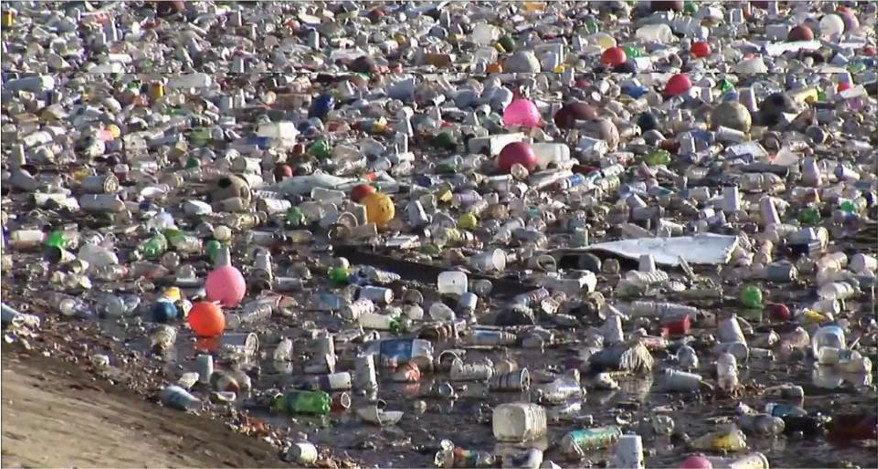
\includegraphics[keepaspectratio=true,width=\iwith]{images/matrix/253_01.jpg}}}&
%
\colorbox{white!0}{ \colorbox{red!70}{
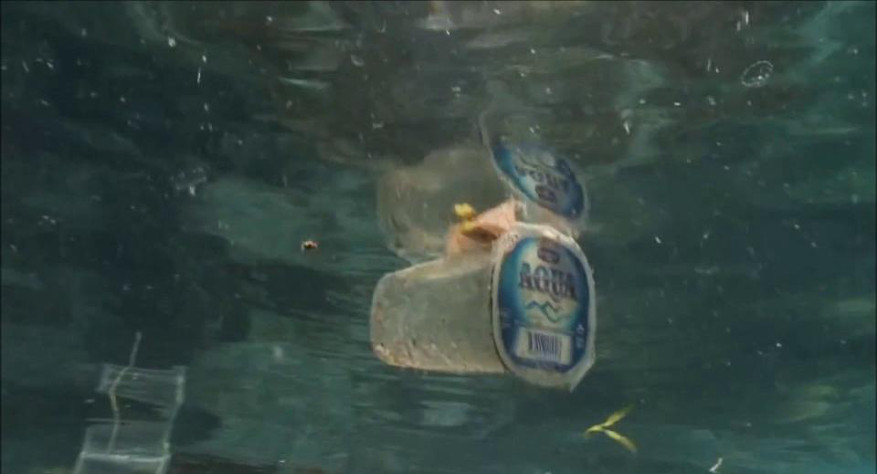
\includegraphics[keepaspectratio=true,width=\iwith]{images/matrix/20607_01.jpg}}}\\
%
\colorbox{white!0}{ \colorbox{white!0}{
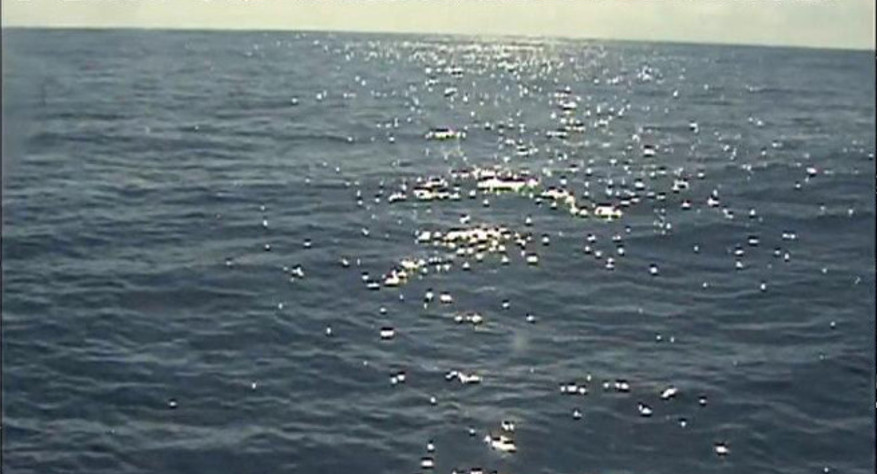
\includegraphics[keepaspectratio=true,width=\iwith]{images/matrix/299_00.jpg}}}&
%
\colorbox{white!0}{ \colorbox{green!80}{
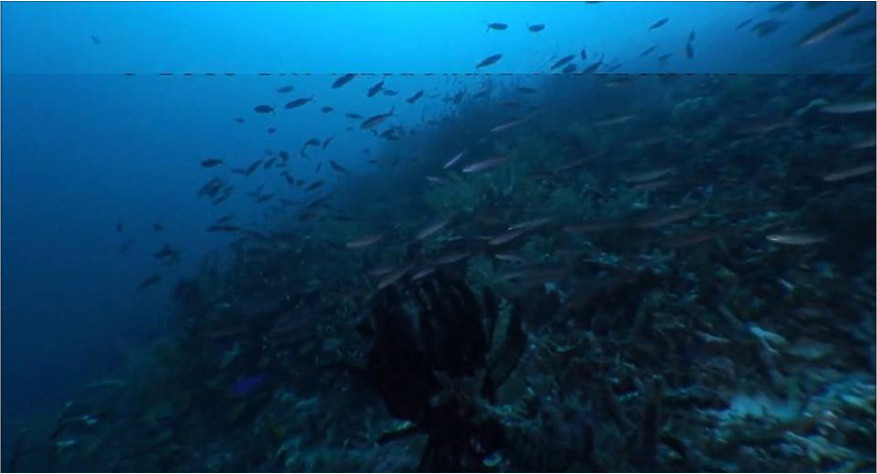
\includegraphics[keepaspectratio=true,width=\iwith]{images/matrix/2737_10.jpg}}}\\
%
\colorbox{red!70}{ \colorbox{green!80}{
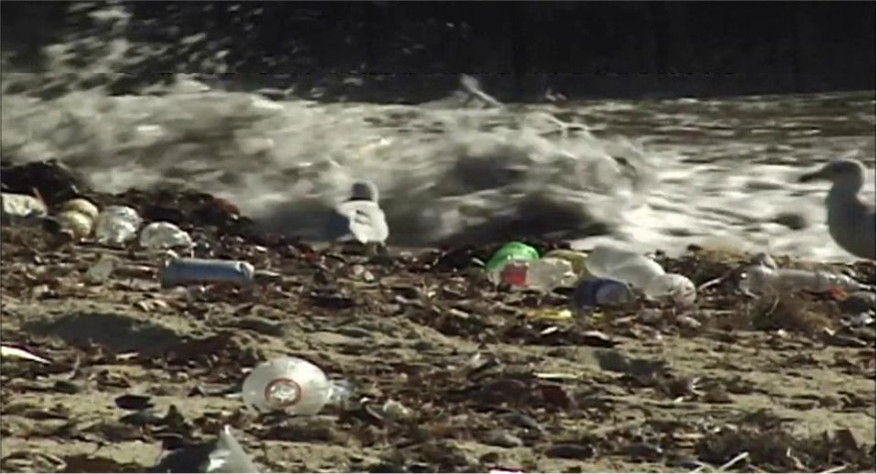
\includegraphics[keepaspectratio=true,width=\iwith]{images/matrix/31_11.jpg}}}&
%
\colorbox{white!0}{ \colorbox{red!70}{
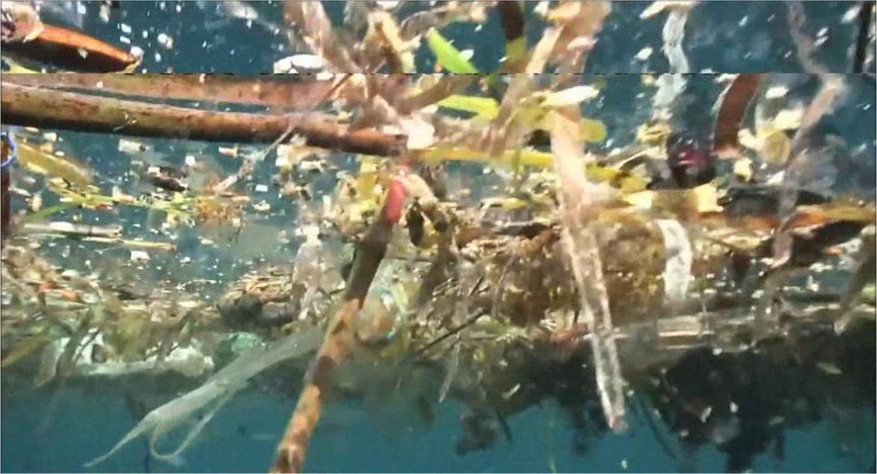
\includegraphics[keepaspectratio=true,width=\iwith]{images/matrix/4409_01.jpg}}}\\
%
\colorbox{white!0}{ \colorbox{green!80}{
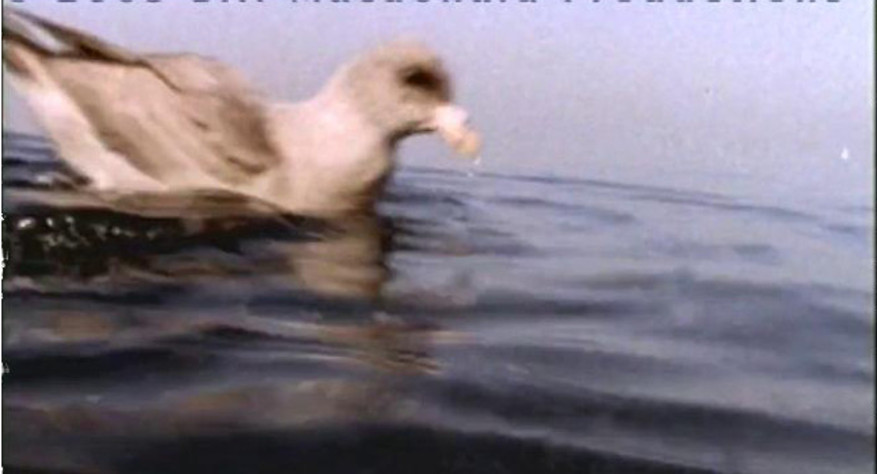
\includegraphics[keepaspectratio=true,width=\iwith]{images/matrix/401_10.jpg}}}&
%
\colorbox{white!0}{ \colorbox{green!80}{
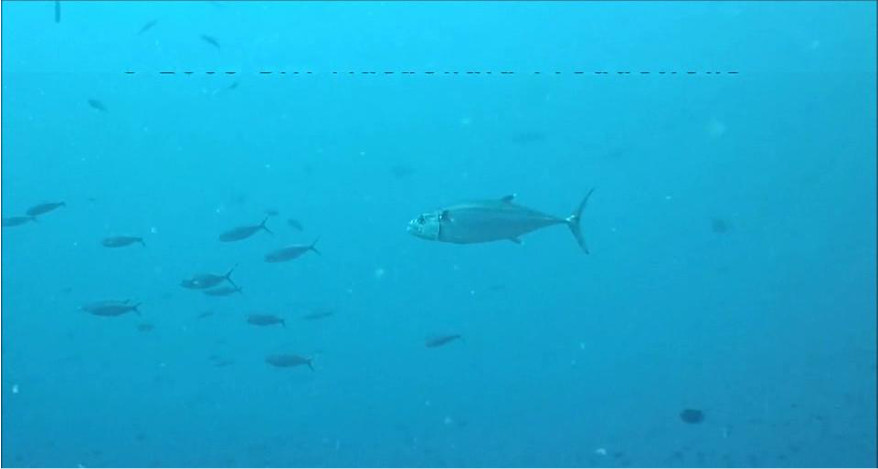
\includegraphics[keepaspectratio=true,width=\iwith]{images/matrix/5053_10.jpg}}}\\
%
\colorbox{red!70}{ \colorbox{green!80}{
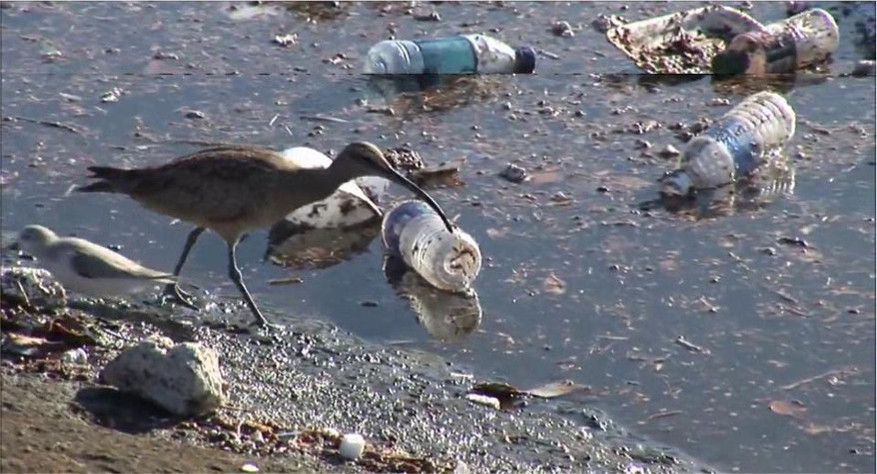
\includegraphics[keepaspectratio=true,width=\iwith]{images/matrix/701_11.jpg}}}&
%
\colorbox{white!0}{ \colorbox{red!70}{
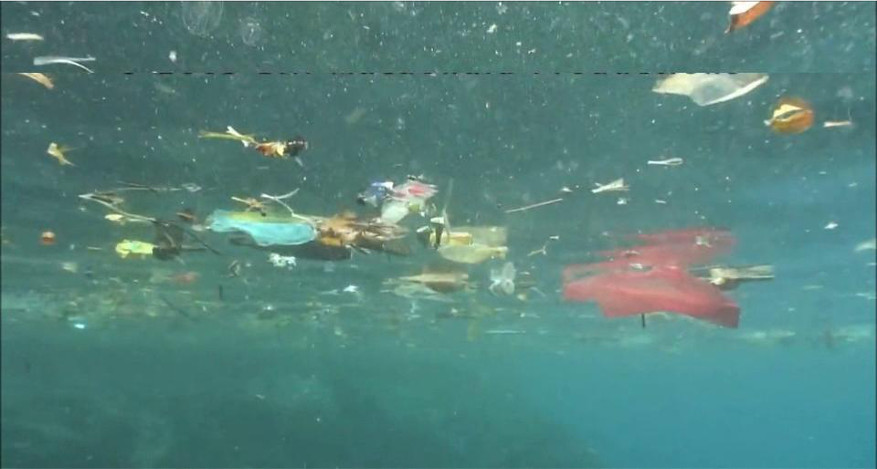
\includegraphics[keepaspectratio=true,width=\iwith]{images/matrix/6_01.jpg}}}
\end{tabular}}
\fi
\caption{Several images from the dataset: Left images are from the above water viewpoint and right images are from below water. A red border indicates an image classified as showing plastic, where a green border indicates an image classified as showing animals.}
\label{fig:datasetimages}
\end{figure}